%! TEX program = lualatex
\documentclass{article}
\usepackage{tikz}
\usepackage[deuteranomaly]{cvd}

\begin{document}

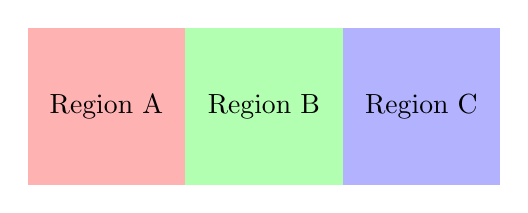
\begin{tikzpicture}
	% Draw a simple map with color-coded regions
	\fill[red!30] (0,0) rectangle (2,2);
	\fill[green!30] (2,0) rectangle (4,2);
	\fill[blue!30] (4,0) rectangle (6,2);

	\node at (1,1) {Region A};
	\node at (3,1) {Region B};
	\node at (5,1) {Region C};
\end{tikzpicture}

\end{document}
